% Created by tikzDevice version 0.12.6 on 2026-08-08 12:10:11
% !TEX encoding = UTF-8 Unicode
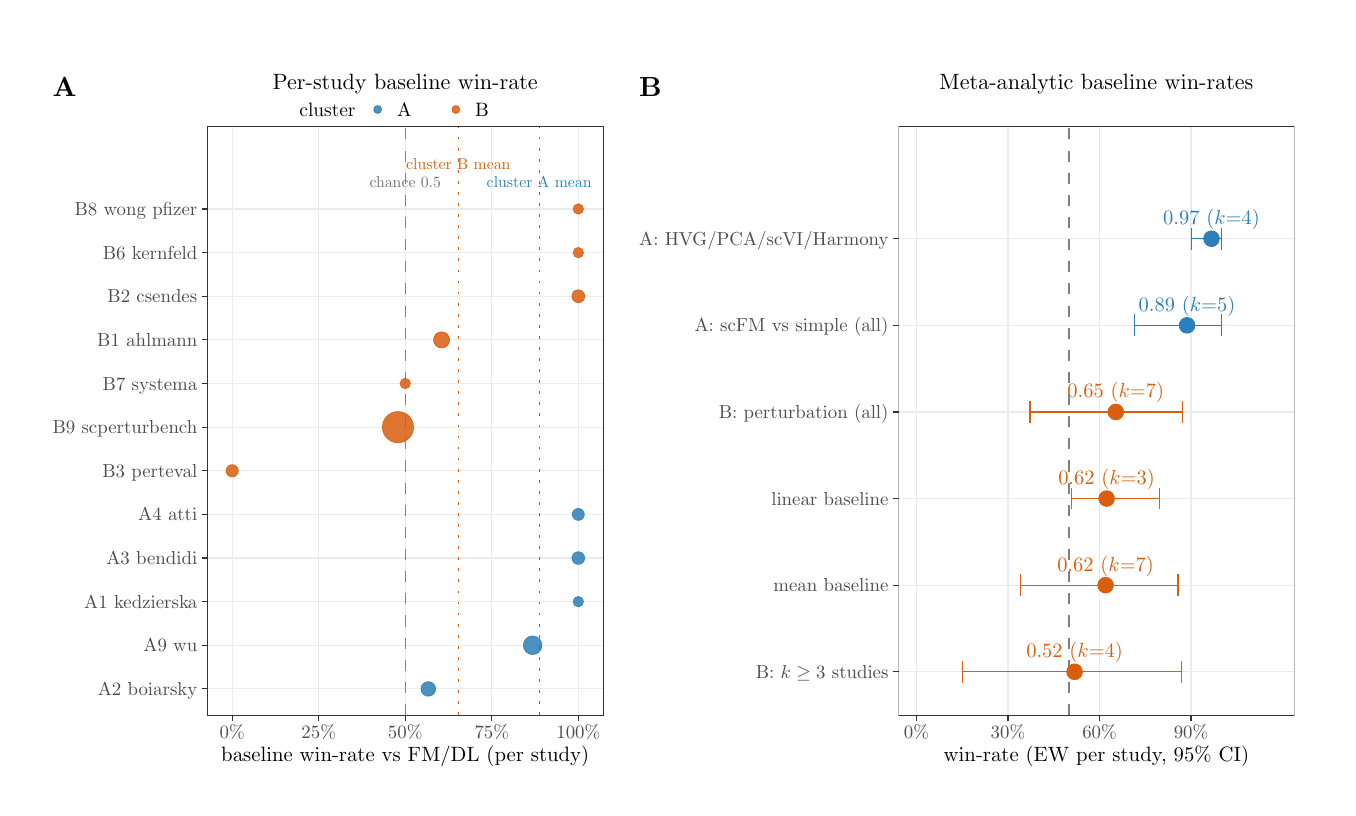
\begin{tikzpicture}[x=1pt,y=1pt]
\definecolor{fillColor}{RGB}{255,255,255}
\path[use as bounding box,fill=fillColor,fill opacity=0.00] (0,0) rectangle (469.75,274.63);
\begin{scope}
\path[clip] (  0.00,  0.00) rectangle (469.75,274.63);
\definecolor{drawColor}{RGB}{255,255,255}
\definecolor{fillColor}{RGB}{255,255,255}

\path[draw=drawColor,line width= 0.4pt,line join=round,line cap=round,fill=fillColor] (  0.00,  0.00) rectangle (469.75,274.63);
\end{scope}
\begin{scope}
\path[clip] (  4.00,  3.00) rectangle (216.98,271.63);
\definecolor{drawColor}{RGB}{255,255,255}
\definecolor{fillColor}{RGB}{255,255,255}

\path[draw=drawColor,line width= 0.4pt,line join=round,line cap=round,fill=fillColor] (  4.00,  3.00) rectangle (216.98,271.63);
\end{scope}
\begin{scope}
\path[clip] (216.98,  3.00) rectangle (463.76,271.63);
\definecolor{drawColor}{RGB}{255,255,255}
\definecolor{fillColor}{RGB}{255,255,255}

\path[draw=drawColor,line width= 0.4pt,line join=round,line cap=round,fill=fillColor] (216.98,  3.00) rectangle (463.75,271.63);
\end{scope}
\begin{scope}
\path[clip] (  0.00,  0.00) rectangle (469.75,274.63);
\definecolor{fillColor}{RGB}{255,255,255}

\path[fill=fillColor] ( 64.89, 26.23) rectangle (207.98,239.06);
\definecolor{drawColor}{gray}{0.92}

\path[draw=drawColor,line width= 0.4pt,line join=round] ( 64.89, 35.69) --
	(207.98, 35.69);

\path[draw=drawColor,line width= 0.4pt,line join=round] ( 64.89, 51.45) --
	(207.98, 51.45);

\path[draw=drawColor,line width= 0.4pt,line join=round] ( 64.89, 67.22) --
	(207.98, 67.22);

\path[draw=drawColor,line width= 0.4pt,line join=round] ( 64.89, 82.98) --
	(207.98, 82.98);

\path[draw=drawColor,line width= 0.4pt,line join=round] ( 64.89, 98.75) --
	(207.98, 98.75);

\path[draw=drawColor,line width= 0.4pt,line join=round] ( 64.89,114.51) --
	(207.98,114.51);

\path[draw=drawColor,line width= 0.4pt,line join=round] ( 64.89,130.28) --
	(207.98,130.28);

\path[draw=drawColor,line width= 0.4pt,line join=round] ( 64.89,146.05) --
	(207.98,146.05);

\path[draw=drawColor,line width= 0.4pt,line join=round] ( 64.89,161.81) --
	(207.98,161.81);

\path[draw=drawColor,line width= 0.4pt,line join=round] ( 64.89,177.58) --
	(207.98,177.58);

\path[draw=drawColor,line width= 0.4pt,line join=round] ( 64.89,193.34) --
	(207.98,193.34);

\path[draw=drawColor,line width= 0.4pt,line join=round] ( 64.89,209.11) --
	(207.98,209.11);

\path[draw=drawColor,line width= 0.4pt,line join=round] ( 73.90, 26.23) --
	( 73.90,239.06);

\path[draw=drawColor,line width= 0.4pt,line join=round] (105.17, 26.23) --
	(105.17,239.06);

\path[draw=drawColor,line width= 0.4pt,line join=round] (136.43, 26.23) --
	(136.43,239.06);

\path[draw=drawColor,line width= 0.4pt,line join=round] (167.70, 26.23) --
	(167.70,239.06);

\path[draw=drawColor,line width= 0.4pt,line join=round] (198.97, 26.23) --
	(198.97,239.06);
\definecolor{drawColor}{gray}{0.50}

\path[draw=drawColor,line width= 0.4pt,dash pattern=on 4pt off 4pt ,line join=round] (136.43, 26.23) -- (136.43,239.06);
\definecolor{drawColor}{RGB}{44,127,184}

\path[draw=drawColor,line width= 0.4pt,dash pattern=on 1pt off 3pt ,line join=round] (184.83, 26.23) -- (184.83,239.06);
\definecolor{drawColor}{RGB}{217,95,14}

\path[draw=drawColor,line width= 0.4pt,dash pattern=on 1pt off 3pt ,line join=round] (155.61, 26.23) -- (155.61,239.06);
\definecolor{drawColor}{gray}{0.45}

\node[text=drawColor,anchor=base,inner sep=0pt, outer sep=0pt, scale=  0.57] at (136.43,216.95) {chance 0.5};
\definecolor{drawColor}{RGB}{44,127,184}

\node[text=drawColor,anchor=base,inner sep=0pt, outer sep=0pt, scale=  0.57] at (184.83,216.95) {cluster A mean};
\definecolor{drawColor}{RGB}{217,95,14}

\node[text=drawColor,anchor=base,inner sep=0pt, outer sep=0pt, scale=  0.57] at (155.61,223.22) {cluster B mean};
\definecolor{drawColor}{RGB}{44,127,184}
\definecolor{fillColor}{RGB}{44,127,184}

\path[draw=drawColor,draw opacity=0.85,line width= 0.3pt,line join=round,line cap=round,fill=fillColor,fill opacity=0.85] (198.97, 67.22) circle (  1.87);

\path[draw=drawColor,draw opacity=0.85,line width= 0.3pt,line join=round,line cap=round,fill=fillColor,fill opacity=0.85] (144.77, 35.69) circle (  2.62);

\path[draw=drawColor,draw opacity=0.85,line width= 0.3pt,line join=round,line cap=round,fill=fillColor,fill opacity=0.85] (198.97, 82.98) circle (  2.28);

\path[draw=drawColor,draw opacity=0.85,line width= 0.3pt,line join=round,line cap=round,fill=fillColor,fill opacity=0.85] (198.97, 98.75) circle (  2.15);

\path[draw=drawColor,draw opacity=0.85,line width= 0.3pt,line join=round,line cap=round,fill=fillColor,fill opacity=0.85] (182.47, 51.45) circle (  3.34);
\definecolor{drawColor}{RGB}{217,95,14}
\definecolor{fillColor}{RGB}{217,95,14}

\path[draw=drawColor,draw opacity=0.85,line width= 0.3pt,line join=round,line cap=round,fill=fillColor,fill opacity=0.85] (149.56,161.81) circle (  2.90);

\path[draw=drawColor,draw opacity=0.85,line width= 0.3pt,line join=round,line cap=round,fill=fillColor,fill opacity=0.85] (198.97,177.58) circle (  2.31);

\path[draw=drawColor,draw opacity=0.85,line width= 0.3pt,line join=round,line cap=round,fill=fillColor,fill opacity=0.85] ( 73.90,114.51) circle (  2.20);

\path[draw=drawColor,draw opacity=0.85,line width= 0.3pt,line join=round,line cap=round,fill=fillColor,fill opacity=0.85] (198.97,193.34) circle (  1.87);

\path[draw=drawColor,draw opacity=0.85,line width= 0.3pt,line join=round,line cap=round,fill=fillColor,fill opacity=0.85] (136.43,146.05) circle (  1.87);

\path[draw=drawColor,draw opacity=0.85,line width= 0.3pt,line join=round,line cap=round,fill=fillColor,fill opacity=0.85] (198.97,209.11) circle (  1.87);

\path[draw=drawColor,draw opacity=0.85,line width= 0.3pt,line join=round,line cap=round,fill=fillColor,fill opacity=0.85] (133.81,130.28) circle (  5.61);
\definecolor{drawColor}{gray}{0.20}

\path[draw=drawColor,line width= 0.4pt,line join=round,line cap=round] ( 64.89, 26.23) rectangle (207.98,239.06);
\end{scope}
\begin{scope}
\path[clip] (  0.00,  0.00) rectangle (469.75,274.63);
\definecolor{drawColor}{gray}{0.30}

\node[text=drawColor,anchor=base east,inner sep=0pt, outer sep=0pt, scale=  0.68] at ( 61.29, 33.35) {A2 boiarsky};

\node[text=drawColor,anchor=base east,inner sep=0pt, outer sep=0pt, scale=  0.68] at ( 61.29, 49.11) {A9 wu};

\node[text=drawColor,anchor=base east,inner sep=0pt, outer sep=0pt, scale=  0.68] at ( 61.29, 64.88) {A1 kedzierska};

\node[text=drawColor,anchor=base east,inner sep=0pt, outer sep=0pt, scale=  0.68] at ( 61.29, 80.64) {A3 bendidi};

\node[text=drawColor,anchor=base east,inner sep=0pt, outer sep=0pt, scale=  0.68] at ( 61.29, 96.41) {A4 atti};

\node[text=drawColor,anchor=base east,inner sep=0pt, outer sep=0pt, scale=  0.68] at ( 61.29,112.17) {B3 perteval};

\node[text=drawColor,anchor=base east,inner sep=0pt, outer sep=0pt, scale=  0.68] at ( 61.29,127.94) {B9 scperturbench};

\node[text=drawColor,anchor=base east,inner sep=0pt, outer sep=0pt, scale=  0.68] at ( 61.29,143.70) {B7 systema};

\node[text=drawColor,anchor=base east,inner sep=0pt, outer sep=0pt, scale=  0.68] at ( 61.29,159.47) {B1 ahlmann};

\node[text=drawColor,anchor=base east,inner sep=0pt, outer sep=0pt, scale=  0.68] at ( 61.29,175.23) {B2 csendes};

\node[text=drawColor,anchor=base east,inner sep=0pt, outer sep=0pt, scale=  0.68] at ( 61.29,191.00) {B6 kernfeld};

\node[text=drawColor,anchor=base east,inner sep=0pt, outer sep=0pt, scale=  0.68] at ( 61.29,206.77) {B8 wong pfizer};
\end{scope}
\begin{scope}
\path[clip] (  0.00,  0.00) rectangle (469.75,274.63);
\definecolor{drawColor}{gray}{0.20}

\path[draw=drawColor,line width= 0.4pt,line join=round] ( 62.89, 35.69) --
	( 64.89, 35.69);

\path[draw=drawColor,line width= 0.4pt,line join=round] ( 62.89, 51.45) --
	( 64.89, 51.45);

\path[draw=drawColor,line width= 0.4pt,line join=round] ( 62.89, 67.22) --
	( 64.89, 67.22);

\path[draw=drawColor,line width= 0.4pt,line join=round] ( 62.89, 82.98) --
	( 64.89, 82.98);

\path[draw=drawColor,line width= 0.4pt,line join=round] ( 62.89, 98.75) --
	( 64.89, 98.75);

\path[draw=drawColor,line width= 0.4pt,line join=round] ( 62.89,114.51) --
	( 64.89,114.51);

\path[draw=drawColor,line width= 0.4pt,line join=round] ( 62.89,130.28) --
	( 64.89,130.28);

\path[draw=drawColor,line width= 0.4pt,line join=round] ( 62.89,146.05) --
	( 64.89,146.05);

\path[draw=drawColor,line width= 0.4pt,line join=round] ( 62.89,161.81) --
	( 64.89,161.81);

\path[draw=drawColor,line width= 0.4pt,line join=round] ( 62.89,177.58) --
	( 64.89,177.58);

\path[draw=drawColor,line width= 0.4pt,line join=round] ( 62.89,193.34) --
	( 64.89,193.34);

\path[draw=drawColor,line width= 0.4pt,line join=round] ( 62.89,209.11) --
	( 64.89,209.11);
\end{scope}
\begin{scope}
\path[clip] (  0.00,  0.00) rectangle (469.75,274.63);
\definecolor{drawColor}{gray}{0.20}

\path[draw=drawColor,line width= 0.4pt,line join=round] ( 73.90, 24.23) --
	( 73.90, 26.23);

\path[draw=drawColor,line width= 0.4pt,line join=round] (105.17, 24.23) --
	(105.17, 26.23);

\path[draw=drawColor,line width= 0.4pt,line join=round] (136.43, 24.23) --
	(136.43, 26.23);

\path[draw=drawColor,line width= 0.4pt,line join=round] (167.70, 24.23) --
	(167.70, 26.23);

\path[draw=drawColor,line width= 0.4pt,line join=round] (198.97, 24.23) --
	(198.97, 26.23);
\end{scope}
\begin{scope}
\path[clip] (  0.00,  0.00) rectangle (469.75,274.63);
\definecolor{drawColor}{gray}{0.30}

\node[text=drawColor,anchor=base,inner sep=0pt, outer sep=0pt, scale=  0.68] at ( 73.90, 17.95) {0\%};

\node[text=drawColor,anchor=base,inner sep=0pt, outer sep=0pt, scale=  0.68] at (105.17, 17.95) {25\%};

\node[text=drawColor,anchor=base,inner sep=0pt, outer sep=0pt, scale=  0.68] at (136.43, 17.95) {50\%};

\node[text=drawColor,anchor=base,inner sep=0pt, outer sep=0pt, scale=  0.68] at (167.70, 17.95) {75\%};

\node[text=drawColor,anchor=base,inner sep=0pt, outer sep=0pt, scale=  0.68] at (198.97, 17.95) {100\%};
\end{scope}
\begin{scope}
\path[clip] (  0.00,  0.00) rectangle (469.75,274.63);
\definecolor{drawColor}{RGB}{0,0,0}

\node[text=drawColor,anchor=base,inner sep=0pt, outer sep=0pt, scale=  0.75] at (136.43,  9.46) {baseline win-rate vs FM/DL (per study)};
\end{scope}
\begin{scope}
\path[clip] (  0.00,  0.00) rectangle (469.75,274.63);
\definecolor{fillColor}{RGB}{255,255,255}

\path[fill=fillColor] ( 97.19,241.06) rectangle (175.68,249.06);
\end{scope}
\begin{scope}
\path[clip] (  0.00,  0.00) rectangle (469.75,274.63);
\definecolor{drawColor}{RGB}{0,0,0}

\node[text=drawColor,anchor=base west,inner sep=0pt, outer sep=0pt, scale=  0.70] at ( 98.19,242.65) {cluster};
\end{scope}
\begin{scope}
\path[clip] (  0.00,  0.00) rectangle (469.75,274.63);
\definecolor{fillColor}{RGB}{255,255,255}

\path[fill=fillColor] (122.47,241.06) rectangle (130.47,249.06);
\definecolor{drawColor}{RGB}{44,127,184}
\definecolor{fillColor}{RGB}{44,127,184}

\path[draw=drawColor,draw opacity=0.85,line width= 0.3pt,line join=round,line cap=round,fill=fillColor,fill opacity=0.85] (126.47,245.06) circle (  1.43);
\end{scope}
\begin{scope}
\path[clip] (  0.00,  0.00) rectangle (469.75,274.63);
\definecolor{fillColor}{RGB}{255,255,255}

\path[fill=fillColor] (150.72,241.06) rectangle (158.72,249.06);
\definecolor{drawColor}{RGB}{217,95,14}
\definecolor{fillColor}{RGB}{217,95,14}

\path[draw=drawColor,draw opacity=0.85,line width= 0.3pt,line join=round,line cap=round,fill=fillColor,fill opacity=0.85] (154.72,245.06) circle (  1.43);
\end{scope}
\begin{scope}
\path[clip] (  0.00,  0.00) rectangle (469.75,274.63);
\definecolor{drawColor}{RGB}{0,0,0}

\node[text=drawColor,anchor=base west,inner sep=0pt, outer sep=0pt, scale=  0.70] at (133.47,242.65) {A};
\end{scope}
\begin{scope}
\path[clip] (  0.00,  0.00) rectangle (469.75,274.63);
\definecolor{drawColor}{RGB}{0,0,0}

\node[text=drawColor,anchor=base west,inner sep=0pt, outer sep=0pt, scale=  0.70] at (161.72,242.65) {B};
\end{scope}
\begin{scope}
\path[clip] (  0.00,  0.00) rectangle (469.75,274.63);
\definecolor{drawColor}{RGB}{0,0,0}

\node[text=drawColor,anchor=base,inner sep=0pt, outer sep=0pt, scale=  0.80] at (136.43,252.12) {Per-study baseline win-rate};
\end{scope}
\begin{scope}
\path[clip] (  0.00,  0.00) rectangle (469.75,274.63);
\definecolor{drawColor}{RGB}{0,0,0}

\node[text=drawColor,anchor=base,inner sep=0pt, outer sep=0pt, scale=  1.00] at ( 13.35,249.75) {\bfseries A};
\end{scope}
\begin{scope}
\path[clip] (314.67, 26.23) rectangle (457.75,239.06);
\definecolor{fillColor}{RGB}{255,255,255}

\path[fill=fillColor] (314.67, 26.23) rectangle (457.75,239.06);
\definecolor{drawColor}{gray}{0.92}

\path[draw=drawColor,line width= 0.4pt,line join=round] (314.67, 41.88) --
	(457.75, 41.88);

\path[draw=drawColor,line width= 0.4pt,line join=round] (314.67, 73.18) --
	(457.75, 73.18);

\path[draw=drawColor,line width= 0.4pt,line join=round] (314.67,104.48) --
	(457.75,104.48);

\path[draw=drawColor,line width= 0.4pt,line join=round] (314.67,135.77) --
	(457.75,135.77);

\path[draw=drawColor,line width= 0.4pt,line join=round] (314.67,167.07) --
	(457.75,167.07);

\path[draw=drawColor,line width= 0.4pt,line join=round] (314.67,198.37) --
	(457.75,198.37);

\path[draw=drawColor,line width= 0.4pt,line join=round] (321.17, 26.23) --
	(321.17,239.06);

\path[draw=drawColor,line width= 0.4pt,line join=round] (354.24, 26.23) --
	(354.24,239.06);

\path[draw=drawColor,line width= 0.4pt,line join=round] (387.31, 26.23) --
	(387.31,239.06);

\path[draw=drawColor,line width= 0.4pt,line join=round] (420.38, 26.23) --
	(420.38,239.06);
\definecolor{drawColor}{gray}{0.50}

\path[draw=drawColor,line width= 0.4pt,dash pattern=on 4pt off 4pt ,line join=round] (376.29, 26.23) -- (376.29,239.06);
\definecolor{drawColor}{RGB}{44,127,184}

\path[draw=drawColor,line width= 0.4pt,line join=round] (431.41,163.16) --
	(431.41,170.99);

\path[draw=drawColor,line width= 0.4pt,line join=round] (431.41,167.07) --
	(399.84,167.07);

\path[draw=drawColor,line width= 0.4pt,line join=round] (399.84,163.16) --
	(399.84,170.99);
\definecolor{drawColor}{RGB}{217,95,14}

\path[draw=drawColor,line width= 0.4pt,line join=round] (417.33,131.86) --
	(417.33,139.69);

\path[draw=drawColor,line width= 0.4pt,line join=round] (417.33,135.77) --
	(362.17,135.77);

\path[draw=drawColor,line width= 0.4pt,line join=round] (362.17,131.86) --
	(362.17,139.69);

\path[draw=drawColor,line width= 0.4pt,line join=round] (416.79, 37.97) --
	(416.79, 45.79);

\path[draw=drawColor,line width= 0.4pt,line join=round] (416.79, 41.88) --
	(337.79, 41.88);

\path[draw=drawColor,line width= 0.4pt,line join=round] (337.79, 37.97) --
	(337.79, 45.79);

\path[draw=drawColor,line width= 0.4pt,line join=round] (415.66, 69.26) --
	(415.66, 77.09);

\path[draw=drawColor,line width= 0.4pt,line join=round] (415.66, 73.18) --
	(358.66, 73.18);

\path[draw=drawColor,line width= 0.4pt,line join=round] (358.66, 69.26) --
	(358.66, 77.09);

\path[draw=drawColor,line width= 0.4pt,line join=round] (408.86,100.56) --
	(408.86,108.39);

\path[draw=drawColor,line width= 0.4pt,line join=round] (408.86,104.48) --
	(377.07,104.48);

\path[draw=drawColor,line width= 0.4pt,line join=round] (377.07,100.56) --
	(377.07,108.39);
\definecolor{drawColor}{RGB}{44,127,184}

\path[draw=drawColor,line width= 0.4pt,line join=round] (431.41,194.46) --
	(431.41,202.28);

\path[draw=drawColor,line width= 0.4pt,line join=round] (431.41,198.37) --
	(420.49,198.37);

\path[draw=drawColor,line width= 0.4pt,line join=round] (420.49,194.46) --
	(420.49,202.28);
\definecolor{fillColor}{RGB}{44,127,184}

\path[draw=drawColor,line width= 0.3pt,line join=round,line cap=round,fill=fillColor] (418.94,167.07) circle (  2.83);
\definecolor{drawColor}{RGB}{217,95,14}
\definecolor{fillColor}{RGB}{217,95,14}

\path[draw=drawColor,line width= 0.3pt,line join=round,line cap=round,fill=fillColor] (393.19,135.77) circle (  2.83);

\path[draw=drawColor,line width= 0.3pt,line join=round,line cap=round,fill=fillColor] (378.30, 41.88) circle (  2.83);

\path[draw=drawColor,line width= 0.3pt,line join=round,line cap=round,fill=fillColor] (389.50, 73.18) circle (  2.83);

\path[draw=drawColor,line width= 0.3pt,line join=round,line cap=round,fill=fillColor] (389.86,104.48) circle (  2.83);
\definecolor{drawColor}{RGB}{44,127,184}
\definecolor{fillColor}{RGB}{44,127,184}

\path[draw=drawColor,line width= 0.3pt,line join=round,line cap=round,fill=fillColor] (427.77,198.37) circle (  2.83);

\node[text=drawColor,anchor=base,inner sep=0pt, outer sep=0pt, scale=  0.74] at (418.94,172.17) {0.89 ($k{=}5$)};
\definecolor{drawColor}{RGB}{217,95,14}

\node[text=drawColor,anchor=base,inner sep=0pt, outer sep=0pt, scale=  0.74] at (393.19,140.87) {0.65 ($k{=}7$)};

\node[text=drawColor,anchor=base,inner sep=0pt, outer sep=0pt, scale=  0.74] at (378.30, 46.97) {0.52 ($k{=}4$)};

\node[text=drawColor,anchor=base,inner sep=0pt, outer sep=0pt, scale=  0.74] at (389.50, 78.27) {0.62 ($k{=}7$)};

\node[text=drawColor,anchor=base,inner sep=0pt, outer sep=0pt, scale=  0.74] at (389.86,109.57) {0.62 ($k{=}3$)};
\definecolor{drawColor}{RGB}{44,127,184}

\node[text=drawColor,anchor=base,inner sep=0pt, outer sep=0pt, scale=  0.74] at (427.77,203.47) {0.97 ($k{=}4$)};
\definecolor{drawColor}{gray}{0.20}

\path[draw=drawColor,line width= 0.4pt,line join=round,line cap=round] (314.67, 26.23) rectangle (457.75,239.06);
\end{scope}
\begin{scope}
\path[clip] (  0.00,  0.00) rectangle (469.75,274.63);
\definecolor{drawColor}{gray}{0.30}

\node[text=drawColor,anchor=base east,inner sep=0pt, outer sep=0pt, scale=  0.68] at (311.07, 39.54) {B: $k\geq3$ studies};

\node[text=drawColor,anchor=base east,inner sep=0pt, outer sep=0pt, scale=  0.68] at (311.07, 70.84) {mean baseline};

\node[text=drawColor,anchor=base east,inner sep=0pt, outer sep=0pt, scale=  0.68] at (311.07,102.13) {linear baseline};

\node[text=drawColor,anchor=base east,inner sep=0pt, outer sep=0pt, scale=  0.68] at (311.07,133.43) {B: perturbation (all)};

\node[text=drawColor,anchor=base east,inner sep=0pt, outer sep=0pt, scale=  0.68] at (311.07,164.73) {A: scFM vs simple (all)};

\node[text=drawColor,anchor=base east,inner sep=0pt, outer sep=0pt, scale=  0.68] at (311.07,196.03) {A: HVG/PCA/scVI/Harmony};
\end{scope}
\begin{scope}
\path[clip] (  0.00,  0.00) rectangle (469.75,274.63);
\definecolor{drawColor}{gray}{0.20}

\path[draw=drawColor,line width= 0.4pt,line join=round] (312.67, 41.88) --
	(314.67, 41.88);

\path[draw=drawColor,line width= 0.4pt,line join=round] (312.67, 73.18) --
	(314.67, 73.18);

\path[draw=drawColor,line width= 0.4pt,line join=round] (312.67,104.48) --
	(314.67,104.48);

\path[draw=drawColor,line width= 0.4pt,line join=round] (312.67,135.77) --
	(314.67,135.77);

\path[draw=drawColor,line width= 0.4pt,line join=round] (312.67,167.07) --
	(314.67,167.07);

\path[draw=drawColor,line width= 0.4pt,line join=round] (312.67,198.37) --
	(314.67,198.37);
\end{scope}
\begin{scope}
\path[clip] (  0.00,  0.00) rectangle (469.75,274.63);
\definecolor{drawColor}{gray}{0.20}

\path[draw=drawColor,line width= 0.4pt,line join=round] (321.17, 24.23) --
	(321.17, 26.23);

\path[draw=drawColor,line width= 0.4pt,line join=round] (354.24, 24.23) --
	(354.24, 26.23);

\path[draw=drawColor,line width= 0.4pt,line join=round] (387.31, 24.23) --
	(387.31, 26.23);

\path[draw=drawColor,line width= 0.4pt,line join=round] (420.38, 24.23) --
	(420.38, 26.23);
\end{scope}
\begin{scope}
\path[clip] (  0.00,  0.00) rectangle (469.75,274.63);
\definecolor{drawColor}{gray}{0.30}

\node[text=drawColor,anchor=base,inner sep=0pt, outer sep=0pt, scale=  0.68] at (321.17, 17.95) {0\%};

\node[text=drawColor,anchor=base,inner sep=0pt, outer sep=0pt, scale=  0.68] at (354.24, 17.95) {30\%};

\node[text=drawColor,anchor=base,inner sep=0pt, outer sep=0pt, scale=  0.68] at (387.31, 17.95) {60\%};

\node[text=drawColor,anchor=base,inner sep=0pt, outer sep=0pt, scale=  0.68] at (420.38, 17.95) {90\%};
\end{scope}
\begin{scope}
\path[clip] (  0.00,  0.00) rectangle (469.75,274.63);
\definecolor{drawColor}{RGB}{0,0,0}

\node[text=drawColor,anchor=base,inner sep=0pt, outer sep=0pt, scale=  0.75] at (386.21,  9.46) {win-rate (EW per study, 95\% CI)};
\end{scope}
\begin{scope}
\path[clip] (  0.00,  0.00) rectangle (469.75,274.63);
\definecolor{drawColor}{RGB}{0,0,0}

\node[text=drawColor,anchor=base,inner sep=0pt, outer sep=0pt, scale=  0.80] at (386.21,252.12) {Meta-analytic baseline win-rates};
\end{scope}
\begin{scope}
\path[clip] (  0.00,  0.00) rectangle (469.75,274.63);
\definecolor{drawColor}{RGB}{0,0,0}

\node[text=drawColor,anchor=base,inner sep=0pt, outer sep=0pt, scale=  1.00] at (225.07,249.75) {\bfseries B};
\end{scope}
\end{tikzpicture}
